\documentclass[lecture.tex]{subfiles}

\begin{document}

\exercice{}
%\video{https://youtu.be/blablabla}
\enonce{rdm-0007}{Portique}


\begin{center}
  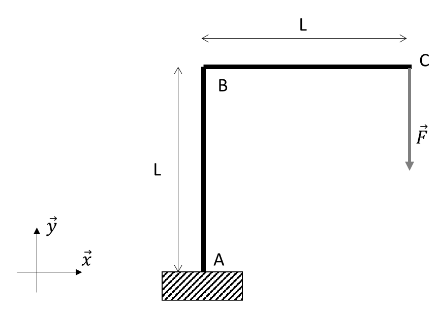
\includegraphics[scale=0.6]{exo-portique-efforts.png}
\end{center}

\begin{enumerate}
  \item Faire le bilan des actions mécaniques extérieures à la poutre.
  \item Déterminer le degré d’hyperstatisme de la poutre.
  \item Trouver les inconnus de liaison de la structure (les efforts et les moments résultants de l’encastrement).
  \item De combien de coupe a-on-t besoin pour étudier les efforts internes
  \item Etudier les efforts internes de la poutre

  \begin{center}
    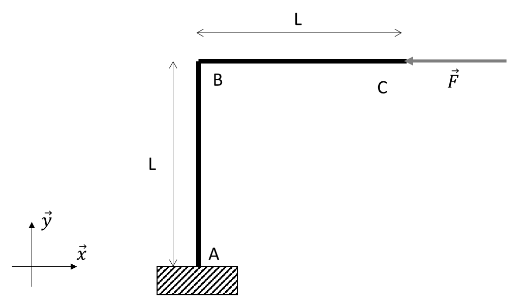
\includegraphics[scale=0.6]{exo-portique-efforts-config2.png}
  \end{center}

  \medskip

  \item Faire le bilan des actions mécaniques extérieures à la poutre.
  \item Déterminer le degré d’hyperstatisme de la poutre.
  \item Trouver les inconnus de liaison de la structure (les efforts et les moments résultants de l’encastrement).
  \item De combien de coupe a-on-t besoin pour étudier les efforts internes
  \item Etudier les efforts internes de la poutre

  \begin{center}
    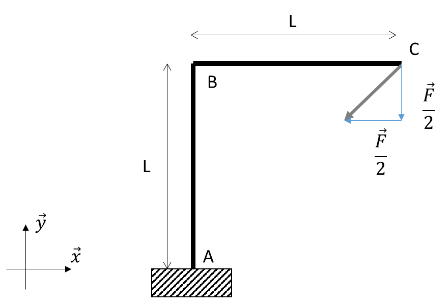
\includegraphics[scale=0.6]{exo-portique-efforts-config3.png}
  \end{center}

  \medskip

  \item Selon vous, est-t-il nécessaire d’après les deux dernières études de refaire le calcul pour trouver les efforts internes dans le cas du portique présenté dans la figure ci-dessus.
  \item Prouvez-le.
\end{enumerate}


\finenonce{rdm-0007}
\finexercice



\end{document}
